% Preamble starts here
\documentclass[utf8,english]{gradu3}

\usepackage{xcolor}
\usepackage{graphicx} % for including pictures

\usepackage{enumitem}
\setlist[itemize]{nolistsep} % smaller gap between nested lists

% NOTE: This must be the last \usepackage in the whole document!
\usepackage[bookmarksopen,bookmarksnumbered,linktocpage]{hyperref}

\addbibresource{thesis.bib}

% My custom macros
\newcommand{\todo}[1]{\textbf{\textcolor{red}{#1}}}
\newcommand{\tmp}[1]{\textit{{#1}}}

%%%%%%%%%%%%%%%%%%%%%%%%%%%%%%%%%%%%%%%%%%%%%%%%%%%%%%%%%%%%%%%%%%%%%%%%%%%%%

% Actual document begins here
\begin{document}

\title{Maintainability in cloud-native architecture}
\translatedtitle{Ylläpidettävyys pilvinatiiveissa arkkitehtuureissa}
\studyline{Software and Telecommunication Technology}
\avainsanat{%
  ylläpito,
  ylläpidettävyys
  julkinen pilvi,
  pilvinatiivi,
  pilviarkkitehti,
  arkkitehtuuri,
  ohjelmistoarkkitehtuuri,
  pro gradu -tutkielmat
}
\keywords{%
  maintenance,
  maintainability,
  public cloud,
  cloud-native,
  cloud architect,
  architecture,
  software architecture,
  Master's Theses}
\tiivistelma{%
  Tutkielman tavoitteena on selvittää kuinka ylläpidettävyys huomioidaan
  pilvinatiivien sovellusten arkkitehtuurisuunnitteluvaiheessa.  Tämän
  saavuttamiseksi suoritan kyselyn Nordcloud-yrityksen pilviarkkitehtien
  keskuudessa.  Ensin määritän kuinka tärkeänä ylläpidettävyyttä pidetään.
  Sitten kategorisoin ehdotukset ylläpidettävyyden huomioimiseen, ja suhteutan
  ne vastaajien kokemuksen määrään kohdealueelta. Lopuksi vertaan kyselyn
  tuloksia kirjallisuudessa ehdotettuihin lähestymistapoihin.
}
\abstract{%
  Goal of the thesis is to investigate how maintainability is addressed during
  the architectural design phase of cloud-native software development lifecycle.
  To this end, I conducted a survey among cloud architects of company Nordcloud,
  where I work.
  First I ascertain the perceived importance of maintainability.
  Then I categorize the suggested approaches for addressing maintainability and
  relate this to the respondents' years of experience in the target domain.
  Finally, I compare the survey results to approaches suggested in the literature.
}

\author{Juho Kettunen}
\contactinformation{\texttt{juho.kettunen@student.jyu.fi}}
\supervisor{Oleksiy Khriyenko}

\maketitle


%%%%%%%%%%%%%%%%%%%%%%%%%%%%%%%%%%%%%%%%%%%%%%%%%%%%%%%%%%%%%%%%%%%%%%%%%%%%%

\begin{thetermlist}
  \item [AD] Architectural Definition
  \item [BaaS] Backend-as-a-Service
  \item [CaC] Configuration as Code
  \item [CI/CD] Continuous Integration, Continuous Delivery/Deployment
  \item [CNA] Cloud-Native Application
  \item [DoS] Denial-of-Service (attack)
  \item [FaaS] Functions-as-a-Service
  \item [IaC] Infrastructure as Code
  \item [MSA] Microservices Architecture
  \item [MVP] Minimum Viable Product
\end{thetermlist}


%%%%%%%%%%%%%%%%%%%%%%%%%%%%%%%%%%%%%%%%%%%%%%%%%%%%%%%%%%%%%%%%%%%%%%%%%%%%%

\mainmatter


%%%%%%%%%%%%%%%%%%%%%%%%%%%%%%%%%%%%%%%%%%%%%%%%%%%%%%%%%%%%%%%%%%%%%%%%%%%%%%
\chapter{Introduction}

Goal of the thesis is to investigate how maintainability should be addressed
during the architectural design of a cloud-native application.  Maintainability
is a quality attribute, which describes how easy it is to maintain and modify a
given system. Software architecture, created by the software architect,
formalizes the structural and behavioral foundation upon which the rest of the
software will be built. Software development life cycle can be described with
different life cycle models that prescribe a way to arrange and order the
different activites of software development. Cloud-nativity means using the
technologies and methods best suited for the cloud computing paradigm. I will
expand upon the relevant terminology in \autoref{chapter:background}.

I aim to answer three research questions:
\begin{itemize}
  \item [\textbf{RQ1}] How much importance do cloud architects place on
        maintainability during the architectural design phase?
  \item [\textbf{RQ2}] How to address maintainability concerns when architecting
        cloud-native applications?
  \item [\textbf{RQ3}] Do the recommendations from literature match the views of
        architects working in the field?
\end{itemize}

The main contribution of this thesis are the results of a survey I conducted in
order to answer the two first research question. The survey was directed at
cloud architects working at my company \textit{Nordcloud}. When analysing
results of the survey, I will first ascertain the perceived importance of
maintainability. Then I will categorize the suggested approaches for addressing
maintainability and contrast this to the respondents' years of experience in the
target domain. Finally, I will compare the survey results to approaches
suggested in literature.

I chose this topic for three reasons. First, the maintenance phase of software
development life cycle is prevalent. It takes up the majority of total lifetime
and costs. \parencite{Bass1998}. Second, choices made during the architectural
design phase cascade into development and maintenance phases. Mistakes and
oversights are slower and more expensive to correct later.
\parencites{Bass1998}{Mumtaz2021}. Lastly, the cloud-native approach is highly
relevant in today's technology landscape. It helps reduce time-to-market and
move costs from capital expenditure to operational expenditure. Utilizing a
public cloud platform also allows the company to leverage a highly scalable,
reliable and secure infrastructure and a wide variety of easily integratable
services. \parencite{Microsoft2022-CNA}.

The thesis is structured as follows. In \autoref{chapter:background} I dive into
related research literature and other contemporary sources to define the
necessary terminology. At the same time, I keep an eye out for best practices
and other suggestions how to most effectively leverage the information in
practice.  Then in \autoref{chapter:method} I describe how my own research is
conducted in regards to the survey and analysis thereof.  The results will be
presented in \autoref{chapter:results}, and further discussed in
\autoref{chapter:discussion}. I will close with conclusions in
\autoref{chapter:conclusions}.


%%%%%%%%%%%%%%%%%%%%%%%%%%%%%%%%%%%%%%%%%%%%%%%%%%%%%%%%%%%%%%%%%%%%%%%%%%%%%%
\chapter{Background}
\label{chapter:background}

\todo{TODO: Review and finalize}

My main database for researching existing literature was the JYKDOK search
engine for international articles \parencite{JYKDOK}.
I decided to search keywords in abstracts, instead of full-text or only in title.
In my opinion the full-text search was too lax, and title-only too strict.
With these search terms I received between 4 to 473 results per search, which
was sufficient:
\begin{itemize}
  \item (Abstract:''cloud native'' AND Abstract:maintainability)
  \item (Abstract:''cloud native'' AND Abstract:architecture)
  \item (Abstract:''cloud native'' AND Abstract:maintenance)
  \item (Abstract:architecture AND Abstract:maintainability AND Abstract:cloud)
  \item (Abstract:serverless AND Abstract:maintainability)
  \item (Abstract:serverless AND Abstract:operations)
  \item (Abstract:''cloud-native'' AND Abstract:quality AND Abstract:attribute)
  \item (Abstract:software AND Abstract:''quality attribute'' AND Abstract:maintainability)
\end{itemize}

To my chagrin, I was unable to find full-text of some articles with promising
abstracts.
In case of one specific article I emailed the authors
\footnote{\textcite{Bogner2018}}, and they kindly sent me a PDF of it.

I also employed an ad-hoc lightweight version of snowballing from bibliographies
of promising sources, e.g. \todo{example here?}

%%%%%%%%%%%%%%%%%%%%%%%%%%%%%%%%%%%%%%
\section{Architecture in software development}

\subsection{Software architecture}

What is software architecture? We can begin by stating that every software
system has one. The architecture exists even if no-one present knows any details
about it \parencite[24]{Bass1998}. \textcite[23]{Bass1998} provide us a
definition as follows:

\begin{quote}
  The software architecture of a program or computing system is the structure or
  structures of the system, which comprise software elements, the externally
  visible properties of those elements, and the relationships among them.
\end{quote}

A \textbf{software system} is a collection of software components organized to
accomplish a specific function or set of functions \parencite[3]{IEEE42010}.
These components --- or elements --- can be entities of varying size: objects,
processes, libraries, databases, commercial software, and so on. In its most
trivial case, we can consider the entire system to be a single component. This
is indeed an architecture, but practically useless due to lack of necessary
details \parencite[24]{Bass1998}. A software architect is a person, team or
organization responsible for systems architecture \parencite[3]{IEEE42010}.

\textcite[53]{Koskimies2005} define a \textbf{component} as an individual
software unit that offers its services through well-defined interfaces.
Implementation details of the components are not considered part of
architecture, but their interactions are. Without describing the interactions we
end up with a ''bubbles and lines'' diagram which is not sufficient to describe
an architecture \parencite[24]{Bass1998}.

A system can comprise more than one structure \parencite[23]{Bass1998}. Because
''structure'' is an abstract concept, it can change depending on perspective. A
\textbf{architectural view} models some aspect of the system
\parencite{Koskimies2005}. It is a representation of a whole system from the
perspective of a related set of concerns, such as a specific stakeholder's
specific concern \parencite[3]{IEEE42010}. A \textbf{stakeholder} is an
individual, team or organization with interests in, or concerns relative to, a
system. Examples include clients, users, the architect, developers, reviewers,
and so on. \parencite[3]{IEEE42010}. Examples of architectural views include a
scenario view, logical view, process view, development view, physical view, and
modification view. They are partly overlapping: when a specific part of a system
is changed, we often need to apply changes in multiple views.
\parencite{Koskimies2005}.

Architecture represents the first design decisions of a system
\parencite{Bass1998}. It is difficult to get it right the first time, and can be
laborious to alter down the road. In worst case, there is a need for an
architectural change, which might result in changes across the entire system and
changes to interaction between components. If we instead can limit the change to
a group of components or only a single one, the change will be easier to carry
out. \parencite[31]{Bass1998}

Out of most design artifacts, architecture has most far-reaching consequences
\parencite[31]{Bass1998}. It will place constraints on implementation and
maintenance: will the system support the required functions; how easy is it to
test, maintain, change and extend; how large data masses can it process, and so
on \parencite{Koskimies2005}.

The architecture might even have effect on the development organization by
nudging towards a specific way to divide tasks to teams by structure of its
components \parencite[31]{Bass1998}. This is somewhat contrary to Conway's law
\footnote{https://en.wikipedia.org/wiki/Conway\%27s\_law} which states that the
technical structure of a system will reflect the social boundaries across the
organizations that produced it. I suppose that in an agile organization the
social structure is malleable enough to be impacted by a new system, when new
teams need to be formed to facilitate the development.

According to \textcite{Koskimies2005}, architecture lies on a higher abstraction
level than implementation. The lower abstraction level of a system manifests as
source code \parencite[24]{Bass1998}. This might be named as ''the
implementation'', or ''design'' as named in \textcite{IEEE12207}. Also
\textcite[4]{IEEE42010} states that architecture is conceptual instead of
concrete. This goes hand in hand with the used vocabulary. With architecture, we
are using the vocabulary of the solution, and are further away from the problem
domain than during implementation \parencite{Koskimies2005}.

When selecting a reference architecture or a fundamental architectural style, we
are dealing with a generic solution that will be further specified later. An
\textbf{architectural style} is a general, high-level guideline for structuring
the components and their responsibilities \parencite[24]{Bass1998}. For example,
client-server architecture is an architectural style. It is not an architecture
in itself: terminology is generic or domain-specific, and the style is not
specific enough to address the requirements set for your new system. Countless
different kinds of architectures can be implemented with the same architectural
style. \parencite[24]{Bass1998}.

As we've read, architecture is of utmost importance for the implementation and
future of the system. Because of this, it seems common sense to document it
somehow. \textcite[24]{Bass1998} define an \textbf{architectural description
  (AD)} as a collection of products to document an architecture
\parencite[3]{IEEE42010}. As such, it is a concrete artifact. They go on to note
that an architecture can live independently of its description or specification
\parencite[24]{Bass1998}. \textcite[27]{Bass1998} outscope the documentation of
guiding processes from actual architecture. In contrast,
\textcite[3]{IEEE42010} mentions ''... and principles guiding its design and
evolution''. The standard states that chosen architectural concepts, as well as
considered alternatives, must be justified in the description. According to
\textcite[67]{IEEE12207}, the description can be utilized at multiple different
levels of abstraction, at each level emphasizing the details necessary for that
level. If an AD is not available, it can be reverse-engineered from an existing
system. This might be needed if, for example, it was originally developed
without a description, or if the original architect is no longer available for
consultation. \parencite[7]{IEEE42010}.

An architecture doesn't spawn out of nothing. Software architecture is based on,
among other things, the requirements placed on it \parencite{Bass1998}.
Requirements codify the collective wishes and needs that various stakeholders
want from the system. If requirements were the only input to software
development, then an identical set of requirements would result in two pieces of
identical architectures, even from two entirely unrelated organizations.
\parencite[5-9]{Bass1998}.

As we can see, the organization, architect or architects, and the technical
environment greatly influence how software systems are built
\parencite{Bass1998}. The organization might have other existing products,
architectures or assets that can be utilized. The organization has some
individual structure, goals and long-term investments, and personnel with
specific skills and availability. Especially the architects' background and
experience is pivotal in deciding the course for the architecture. The architect
might lean on a familiar architectural style that they have had success with in
the past, and vice versa with an unhappy experience. Their professional
community can infuse into the new system a set of standard industry practices
and software engineering techniques. \parencite[5-9]{Bass1998}.

The architecture cause feedback to its background factors, such as the
organization, customers, architects and the software engineering culture in
general \parencite{Bass1998}. Because an architecture dictates the structure of
a software system, it influences the structure of the development project with
respect to team formation, schedules and budgets. If the architecture is seen as
successful, it might be used in future projects, and then the team structure
might become a permanent part of the organization. The software might also offer
a foothold in a certain market area, and this way the organization could update
its goals to take advantage of this new possibility. Customers will likely grow
fond of a good software product, which lowers the threshold for reusing a
battle-tested architecture, because this is more economical than building a new
one from scratch. The architects themselves gain more experience from this
specific system, which means that the system's success or failure will affect
architectural choices made in future projects. When looking through a wider
lens, an especially novel and successful architecture might influence the
software engineering culture as a whole, outside of the organization from which
is sprung. Imagine, for example, the tides created by the first relational
databases, spreadsheets, windowing systems, or WWW itself.
\parencite[10-11]{Bass1998}.


\subsection{Software development life cycle}

Every software system has a life cycle \parencite[17]{IEEE12207}. A \textbf{life
  cycle model} is a framework that contains the processes, activities and tasks
used during the life of the system, from initial requirements gathering to the
termination of its use \parencite[3]{IEEE42010}. The specific life cycle stages
depend on the chosen life cycle model, of which there are many to choose from:
incremental, spiral, iterative, evolutionary, and so on. Usually there is an
initial planning stage, where the need for a new software system arises. After
the need is verified, requirements are gathered. Next there might be a
prototyping phase where multiple architectures are rapidly mocked and evaluated.
Once a rough architectural direction is chosen, an initial architectural
definition is formed. After it is validated, there often follows an iterative
cycle where analysis, design, implementation, verification, validation and
delivery are repeated and intertwined. \parencite[18]{IEEE12207}.

\textcite{Koskimies2005} suggest an architecture-oriented software development
process. It highlights architectural design and evaluation as a crucial life
cycle stage before moving onto detailed design and implementation. Architecture
should be devised incrementally and iteratively from the requirements most
relevant to architecture. Usually it is good to start from functional
requirements, after which the non-functional qualities must be pursued.
\parencite{Koskimies2005}.

In this thesis I don't cling to any particular software lifecycle model.
Instead we rely on the general notion that the initial architecture definition
and architectural design happens early on in the life cycle of a software
system. Naturally, the requirements, architecture or detailed design might need
refinement also later on during operations and maintenance when using an
iterative life cycle model \parencite{IEEE12207}. We will focus on the early
choices and design decisions that influence the activities for the rest of the
software lifecycle. We can call these architectural activities as
''architecting'', which comprises defining, documenting, maintaining, improving
and certifying proper implementation of an architecture
\parencite[3]{IEEE42010}. In addition to these architecting activities,
\textcite[12]{Bass1998} mention creating a business case for the system, and
implementing the system based on the architecture.

\textcite{IEEE12207} defines processes related to architecture and design. Next
we will make a distinction between two related but separate processes: the
\textbf{Architectural Definition process}, and the Design Definition process.
The purpose of the Architectural Definition process, as outlined in
\textcite[66]{IEEE12207}, is threefold. First, the architect should create
alternatives for a system's architecture. Then, we should choose one or
multiple alternatives that properly frame the stakeholders' needs and fulfill
the requirements placed on the system. Lastly, all of this should be described
with a set of uniform views.

At a lower abstraction level, the \textbf{Design Definition process}
\parencite[71]{IEEE12207} is supposed to provide enough detailed data and
information about the system and its components for implementation to be in line
with the architectural entities. It involves preparing for software system
design definition by e.g. prioritizing design principles and characteristic,
identifying and planning for necessary enabling systems and services, and
obtaining access to those enabling systems or services. Then we should establish
designs related to each software element. This goes deep in the technical
details, such as database structures, provisions for memory and storage,
software processes, and external interfaces. \parencite[72]{IEEE12207}. In this
thesis I consider this realm of ''design'' or ''detailed design'' to belong to
software developers instead of architects.

As we've discussed before, architecture is at a higher level of abstraction than
design \parencite{IEEE12207}. Architecture focuses on suitability, viability and
desirability that the architecture is supposed to provide. Meanwhile, design is
focused on compatibility with technologies and other design elements, and
feasibility of implementation and integration. An efficient architecture is as
design-agnostic as possible, to provide most flexibility in planning the said
design. \parencite[71]{IEEE12207}. Because ''design'' is such an ambiguous word,
in this thesis I will use it in accordance to the definition from
\textcite{IEEE12207} as an activity separate from architecting, unless used in
conjunction with with ''architectual'', as in ''architectual design''.

According to \textcite[71-72]{IEEE12207}, selecting the technologies for
implementation and considering compatibility with technologies also falls under
the Design Definition process. In my experience with public cloud providers such
as Amazon Web Services, Microsoft Azure and Google cloud, implementation
technologies are at least to some degree decided by architects instead of
software developers. The architect wants to know which cloud platform is
required or preferred by the customer, in order to reduce the technology space
to a reasonable set of alternative services provided by the platform. The
architect can then work with the available services to compose an architecture
that best serves the stakeholders' needs. The finer details, such as the choice
of programming language or code-level design patterns, can be left to software
developers, as also implied by the ISO/IEC standards.

\textbf{Maintenance stage} is a phase in software life cycle that is often
considered less glamorous than working on greenfield projects and building the
next software hit. Despite this, it is generally accepted that a substantial
portion of the total cost of software is spent on maintenance.
\textcite[32]{Bass1998} go as far as to say this figure is close to 80\%.
Obviously the actual numbers might be slightly different these days 25 years
after their estimate, but the implication holds: considering maintenance efforts
as early as possible in the software life cycle can pay off.
\textcite[1]{Mumtaz2021} echo that architectural issues should be tackled in a
timely manner, because the cost of fixing those kinds of problems later can be
exceptionally high.

\textcite{IEEE12207} outlines the \textbf{Maintenance process}, which in general
comes later in the life cycle after Architectural Definition and Design
Definition processes. Its purpose is to sustain the capability of the system to
provide a service. This can be achieved by monitoring the system's capability to
deliver services; recording incidents for analysis; taking corrective, adaptive,
perfective and preventive actions; and confirming restored capability. In
practice, preparing for maintenance should begin already during architecting. It
is necessary to consider constraints placed on the architecture by
maintenance-related requirements. This can be done, for example, by emphasizing
encapsulation, modularity, and scalability. Documenting the architecture and
system reduces the efforts required to reverse-engineer the system and
components when a fix is needed. The decisions made during architecting can also
affect the need and possibilities for e.g. remote diagnostics and maintenance,
roll back, backup, and recovering data. \parencite[95-96]{IEEE12207}.

Tasks performed during maintenance activities vary between systems and
organizations. There is a need to review stakeholder requirements, complaints,
events, incident and problem reports in order to identify the type of
maintenance effort needed \parencite{IEEE12207}. If the organization has adopted
an iterative software life cycle model, software requirements might change
during maintenance. This change in requirements can be a source for adaptive and
perfective maintenance activities. In that case there will be a need to make
corrections, improvements or other changes to software that is already deployed
\parencite[97]{IEEE12207}. As \textcite[32]{Bass1998} points out, having a good
grasp of the architecture will help manage changes and reason about them.


\subsection{General advice for achieving a good architecture}

Because every system has an architecture, you can create an architecture through
the simple method of trial and error. Unfortunately, an architecture built this
way is unlikely to fulfill the requirements and goals placed on it
\parencite[24]{Bass1998}. He outlines some helpful advice for creating an
architecture from the correct principles. These rules of thumb are divided into
two categories: process-related and structure-related advice.

First we will delve into the \textbf{process-related} topics. As a general rule,
there should be a single architect or a team of architects with a designated
leader \parencite[15]{Bass1998}. Functional requirements and a prioritized list
of quality attributes should be listed, so that the architecture can be steered
towards achieving them. The architecture should be formally evaluated for
quality attributes, and analyzed for applicable quantitative measures, such as
maximum throughput. Having an architecture support iterative implementation
makes integration and testing easier: a ''skeleton system'' can prove that
component communication works, even with otherwise minimal functionality. The
architect is also responsible for defining, distributing, maintaining and
enforcing resource constraints to the responsible implementation teams. For
example, there might be limits to network traffic or hardware performance that
the teams must heed. A good documentation is also a must, with at least one
static view and one dynamic view, written in a notation that all stakeholders
can understand with minimal effort. Speaking of stakeholders, they should be
actively participating in evaluating the architecture, to ensure their needs are
being met. \parencite[15]{Bass1998}.

Next up are the \textbf{structure-related} pieces of wisdom.
\textcite[16]{Bass1998} state that modules should be well defined, with a clear
separation of concerns and following the principles of information hiding. Their
interfaces should also be well defined, and encapsulate any details that might
change during implementation, such as choice of data structures. To improve
modifiability, the modules that produce data should be kept separate from those
that consume data. Between the modules, there should be only a small set of
different ways of interaction, which is to say, the system should perform
similar tasks in a similar fashion all around. This helps improve
understandability, reliability and modifiability, with an added benefit of
shorted development time and conceptual integrity of the architecture. Each
quality attribute should be strived towards with well known architectural
tactics that suit it. The architecture should not depend on any specific version
of a commercial product or tool, or if it does, changing the product or tool
should be both straightforward and cheap. If working close to hardware, changing
the processor allocated for each task or process should be easy even at runtime.
In case of parallel-processing systems, special care should be given to
processes or tasks that touch multiple modules. \parencite[16]{Bass1998}.


%%%%%%%%%%%%%%%%%%%%%%%%%%%%%%%%%%%%%%
\section{Maintainability}

\subsection{Quality Attributes}

The main goal of software development is software of high quality. We of course
expect that the system fulfills all its requirements, gives us correct and
accurate results, and that it interacts with other systems in an expected manner
\parencite[76]{Bass1998}. According to \textcite[602]{Gorla2010}, this quality
can be influenced by factors that are \textbf{organizational},
\textbf{technological}, or \textbf{end user-related}. Organizational factors can
include the IT budget, number of people in system development in that
organization, and quality of documentation. Level of user involvement and user
training the systems are end user-related factors. In contrast, technological
factors include experience and skill level of the development staff, and type
and suitability of development method, programming language or database model.
\parencite[602]{Gorla2010}. Few factors outside the technological category are
relevant in this thesis, which is why I mostly -- although not exclusively --
focus on factors that can be influenced by the software architect.

\textbf{Quality attributes} are used to describe specific aspects of quality as
it relates to software. From management perspective, we are likely interested in
business-related attributes and metrics such as cost and effort of development
work, productivity estimation, and time-to-market
\parencites[60]{Arvanitou2017}[76]{Bass1998}. In this thesis I only deal with
these topics at a superficial level, as they cannot be directly quantified based
on architecture alone. \textcite[76]{Bass1998} suggest that there are two
categories of quality attributes that instead can be measured on architectural
level: attributes that \textbf{can be observed by running the system}, and those
that cannot. The first category tells us how well the system fills its
behavioral requirements during runtime. Quality attributes that indicate this
include \parencites[79-81]{Bass1998}[13]{Li2021}[60]{Arvanitou2017}:
\begin{itemize}
  \item performance
  \item security
  \item availability
  \item functionality
  \item usability
  \item monitorability
  \item reliability
  \item safety
  \item fault prediction
  \item defect proneness
\end{itemize}

The second category of quality attributes --- those that \textbf{cannot be
  observed by running the system} --- tell us how easy the system is to test,
integrate and modify \parencite[81]{Bass1998}. It contains, among others, these
attributes:
\begin{itemize}
  \item modifiability
  \item portability
  \item reusability
  \item integrability
  \item testability
\end{itemize}

Other authors use related terms ''functional'' and ''non-functional
requirements''. \textcite[76]{Bass1998} consider this dichotomy useless. It
suggests that all attributes can be divided strictly into those that model the
system's ability to perform the actions it is expected to, and ''everything
else''. The latter non-functional category acts as a bucket. This too easily
leads to a situation where some qualities are given less consideration, leading
to a diminished quality of the system as a whole. In fact, many quality
attributes are intertwined to behavior of the system. For example, it might be
impossible to reach lightning fast performance with a feature that processes
very large images. On a higher level, though, Bass and others consider
functionality to be orthogonal to quality attributes. If this wasn't the case,
implementing a certain functionality would always dictate the system's security,
usability, or other attributes. The program might function perfectly, but it
might also be difficult to modify or costly to build. \parencite[77]{Bass1998}.

Instead, architectural choices made by the architect decide the level of quality
possible for the system \parencite[72]{Bass2003}. Quality must be considered at
every stage of design, implementation and deployment \parencite{Bass1998}.
Different quality attributes represent themself differently at different stages.
For example, some usability decisions, such as details of a UI, are not
architectural at all. Modifiability, on the other hand, is primarily
architectural. Modifiability relates to how a system is split into components,
and a system is modifiable if changes do not require touching multiple
components. Performance depends on both architectural and non-architectural
considerations. Architect can influence how functionality is divided between
each component, and how they communicate. But the finer details are left to
developers, who are usually responsible or detailed design. An example of this
is the choice of an algorithm and turning it into source code. Another thing to
consider is that quality attributes do not exists in a vacuum, but instead
influence each other in good or bad \parencite[78]{Bass1998}. For example,
improved monitorability likely enables improved testability, which in turn leads
to an increase in security \parencite[18]{Li2021}. Architect must prioritize the
quality attributes and decide which ones to emphasize \parencite[129]{Bass1998}.


\subsection{What is maintainability, and why is it important}

The quality attribute \textbf{maintainability} describes the efforts needed to
fix errors or to make enhancements to the system \parencite[603]{Gorla2010}.
Based on their mapping study on design-time quality attributes and metrics,
\textcite{Arvanitou2017} found that maintainability is the most often researched
quality attribute in most stages of the software development life cycle. It
receives interest in design, architecture, implementation and maintenance
stages. Maintainability is especially relevant in other stages such as project
management, requirements or testing stages. \parencite[61-62]{Arvanitou2017}.

Like many other quality attributes, maintainability can be further subdivided
into more specific quality attributes. \textcite[233]{ISO5055} lists
\textbf{modularity}, \textbf{reusability}, \textbf{analyzability},
\textbf{changeability}, \textbf{modification stability}, \textbf{testability}
and \textbf{compliance} as components of maintainability. Many of these are also
echoed by \textcite[61]{Arvanitou2017}. Some other categories, such as
\textbf{understandability}, are sometimes related to maintainability.
\textcite{Arvanitou2017} consider it a separate quality attribute for two
reasons. First, some other quality models make a distinction between
maintainability and understandability. Second, a unique research community has
already gathered around understandability as a standalone concept.
\parencite[61]{Arvanitou2017}.

There is no single metric ''maintainability of the software system'', because
its components likely have different purposes and implementations
\parencites[26]{Broy2006}[192]{Bass1998}. As such, a phrase like ''the system is
highly maintainable'' doesn't tell anything practical about the system, because
quality attributes receive their meaning from surrounding context. For example,
the software might be highly modifiable in relation to specific classes of
changes. \parencite[192]{Bass1998}.

Focusing on maintainability can pay back the cost invested into it. It
influences how much money and time needs to be spent on maintenance tasks
\parencite[21]{Broy2006}. If it is not considered, cost of change can be
unnecessarily inflated \parencite[2]{Vale2022}. Personnel requirements have to
also be considered, because someone needs to perform necessary updates and
fixes. \textcite{Heroku2011} warns that if maintenance work is left to the one
single team of software developers, the time is often deducted from development
of new features.

If a system is not maintainable, it will be more difficult to address other
problems, such as performance or reliability \parencite[46]{Bouwers2010}. If
different services are coupled, one of them cannot be altered without changing
others that are depending on it \parencite[2]{Vale2022}. At the business level,
maintainability of an important system defines the organization's ability to
adapt their business processes to changing market circumstances, and to
implement innovative products and services \parencite[21]{Broy2006}.

Even if the software itself stays unchanged for years, it can break if and when
its environment changes. This phenomenon is called \textbf{software rot}
\footnote{\url{http://www.catb.org/jargon/html/S/software-rot.html}.}. In other
words, software rot happens when a system's assumptions go out of date. A good
example of this is the infamous ''Y2K'' event which resulted in uncountable bugs
when two-digit year counters underwent wrap-around at the start of the new
millennium. Even outside such one-off situations, software can touch the
underlying operating system and network infrastructure in many places: library
versions, directory paths, IP addresses and hostnames, and so on
\parencite{Heroku2011}. The above Jargon File \footnote{The Jargon File is a
  ''comprehensive compendium of hacker slang illuminating many aspects of hackish
  tradition, folklore, and humor.''
  \url{http://www.catb.org/jargon/html/online-preface.html}} entry about software
rot advises to employ robust design to deflect such problems. Based on what
we've discussed in this chapter, I consider taking care of maintainability part
of robust design.


\subsection{How to measure maintainability}

\todo{think: is this section necessary, either in this depth or at all?}

As discussed before, problems discovered early in the software development life
cycle are easier to address \parencite{Bass1998}. At that point you still have a
chance to adjust requirements, specification or design with relatively low cost.
Software quality cannot be ''appended'' to the project afterwards, but must
instead be baked in deliberately. Qualities of a system can be anticipated by
evaluating the architecture. This means we should evaluate the architecture as
soon as feasible. To evaluate a certain quality attribute, we must make sure we
have the necessary architectural descriptions at hand. For example when
evaluating modifiability --- a subcategory of maintainability --- we need at
least a decomposition that shows us the different modules and how tasks are
distributed between them. \parencite[32, 190-191]{Bass1998}.

It is necessary to decouple quality attributes from effort estimations in our
daily work. \textcite{Moses2009} points out that maintainability of a software
module is intended to signify possible challenges posed by code for maintenance
tasks. Maintainability cannot give you an estimate of how difficult a certain
maintenance change will be or how long it will take. Unless the same change has
been performed in exactly the same circumstances before, duration and
possibility of success of a code change are only subjective estimates. Moses
suggests two methods for estimating practical maintenance tasks. It can be given
on an ordinal scale of e.g. 1-5 instead of an absolute time estimate. If a
concrete estimate is necessary, two experts should voice their opinions, from
which we can calculate an expected duration with confidence limits.
\parencite[204]{Moses2009}.

Vice versa, a prediction system for maintenance effort is not a prediction
system for the quality attribute maintainability \parencite[206]{Moses2009}.
Each maintenance effort includes factors that influence the duration of the
activity. These factors include availability of documentation, amount of
testing after the change, and skills of the maintenance team. Because it is
obviously impossible to carry out and measure all possible maintenance
activities for a system, the effort can only be measured from a subset of all
possible maintenance activities. This means that, even in the best scenario, a
system's maintainability can be estimated only for activities that are similar
to ones that have already been performed before to this system. In the worst
case, the measured effort can be misleading, if measured activities do not
represent actions that are carried out in practice. \parencite[206]{Moses2009}.

\textcite{Broy2006} state that an evaluation criteria must be well-founded and
checkable. Evaluating a whole software system is quite involved, and requires
multiple kinds of evaluation methods. Source code can be automatically checked
for syntactical properties. Other methods are semi-automatic, requiring some
human actions. The rest are thoroughly manual, such as reviewing documentation,
or evaluating whether the system employs correct data structures
\parencite[22]{Broy2006}. Our focal point of interest, maintainability, is a
high-level quality attribute, because it cannot be directly calculated from
metrics \parencite[60]{Arvanitou2017}.

There are ways to measure maintainability indirectly. In their study about
designing microservice systems using patterns, \textcite[9]{Vale2022} found that
the participating industry experts do not measure quality attributes directly.
Instead, they measure quality attributes as a sum of lower-level attributes or
processes related to the quality attributes in question. These lower-level
attributes include measuring code coverage, time taken to resolve issues, and
analysis of architectural debt, which all are indirect metrics for
maintainability. Vale and others reason that this might be because lower level
attributes are easier to measure and check directly than maintainability. They
also postulate that subjective understanding of quality attributes is very much
personal and often vague. This makes it difficult to mutually agree on a
definition inside your organization. Instead, participants rather liked to think
directly of techniques and tools to tackle the related problems.
\parencite[7-10]{Vale2022}.

Automatic methods for assessing maintainability of a system usually limit
themselves to the source code level. Such methods cannot be used to to evaluate
an architecture before implementation has taken place. They are, however, useful
after the fact, for example when following an iterative life cycle model.
\textcite[1]{ISO5055} points out that faults in architectural or design practice
can also be detected by statically analysing design specifications. This
requires that the specification is written in a design language with a formal
syntax and semantics. \textcite[2]{ISO5055} presents a long list of
\textbf{Automated Source Code Quality Measures (ASCQM)}, that provide strong
indicators for the quality of a software system in each area. In my opinion,
these are the architecture-related maintainability \textbf{weaknesses}
\parencite[38-47]{ISO5055}:
\begin{itemize}
  \item invocation of a control element at an unnecessarily deep horizontal
        layer (layer-skipping call)
  \item invokable control element with excessive file or data access operations
  \item invokable control element with large number of outward calls (excessive coupling
        or fan-out)
  \item modules with circular dependencies
\end{itemize}

The standard also provides multiple \textbf{detection patterns}
\parencite[2]{ISO5055}. They help detect structural weaknesses from code. One
pattern can be used to detect multiple weaknesses. I would list the following
maintainability detection patterns as related to architecture
\parencite[48-54]{ISO5055}:
\begin{itemize}
  \item limit number of data access
  \item limit number of outward calls
  \item ban circular dependencies between modules
\end{itemize}

\textcite[63]{Arvanitou2017} note that there are two categories of metrics for
quantifying quality attributes: those that can be evaluated through a single
metric, and those evaluated with multiple. \textcite[66]{Arvanitou2017} list the
following metrics relating to the architectural stage:
\begin{itemize}
  \item cyclomatic complexity
  \item coupling factor
  \item coupling between objects
  \item number of modules
  \item information flow (fan-out)
  \item non-functional coverage
  \item absolute adaptability of a service
  \item relative adaptability of a service
  \item mean of absolute adaptability of a service
  \item mean of relative adaptability of a service
  \item level of system adaptability
\end{itemize}

Most of the tools to calculate these metrics are unnamed, likely created in
academia by research teams, and not available for public use
\parencite{Arvanitou2017}. Maintainability is often connected to metrics, but is
not always quantified as their function. Evaluating a quality attribute with a
single function is non-trivial, which is why few research have suggested such a
function for high-level attributes like maintainability.
\parencite[67]{Arvanitou2017}.

In regards to software, a ''\textbf{smell}'' is considered synonymous to
antipattern, flaw or anomaly \parencite[1]{Mumtaz2021}. In their paper about
architectural smells detection, \textcite[20]{Mumtaz2021} found that research
tends to focus on dependency smells. Dependency smells are usually connected
with coupling issues in the architecture, which relates to maintainability. Most
detection tools can detect common dependency smells. They describe the different
approaches to detect architectural smells in a software system
\parencite[8-14]{Mumtaz2021}:
\begin{itemize}
  \item  graph-based
  \item design structure matrix
  \item model-driven
  \item code smells analysis
  \item reverse engineering and history-based
  \item search-based
  \item visualization
  \item rules-based
\end{itemize}

\textbf{Graph-based} approach depicts system's components as nodes, and their
relationships as edges \parencite{Mumtaz2021}. This makes it easy to notice
problematic relationships between them. A \textbf{design structure matrix} is a
two-dimensional matrix to represent the structural relationships of the
software. This can be used to represent complex architectural components and
their relationships. \textbf{Model-driven} approach represents structure and
behavior of a system using abstractions and modeling. \textbf{Search-based}
methods such as genetic programming are suitable for especially large datasets,
and a \textbf{visualization} approach can help us understand large software
systems with multivariate and multidimensional data.
\parencite[9-14]{Mumtaz2021}.

\textbf{Rules-based} approach takes advantage of metrics their thresholds and
predefined frameworks, heuristics or guidelines \parencite[8]{Mumtaz2021}. It is
related to code smells analysis, which combs through source code to identify
code smells in order to detect architectural smells from them. This approach can
find a correlation between subjective experiences and economical facts of the
system \parencite[22]{Broy2006}. Downsides to a rules-based approach is that it
concentrates on features that can be calculated automatically from source code,
which restricts it to syntactical factors. Automatic checking is difficult to
employ when scrutinizing suitability of data structures, or quality of
documentation. Standards and guidelines might be too generic to be evaluated.
This is a problem if there is no way to concretely check the impact or value of
an attribute, such as modifiability. Some guidelines might also lack reasoning
for the presented advice. Consider the proposition to keep method length to
under 30 lines of source code. Why 30? Who not 25 or 37? Without a solid
argument, the advice will likely stay unheeded. The approach also requires the
user to additionally consider the organizational context for the automatically
calculated result, or else it is useless in evaluating maintainability of the
system as a whole. \parencite[22]{Broy2006}.

\todo{summary? how to best measure? is it even relevant to the research questions?}

\subsection{How to improve maintainability}

There will be less need to reverse-engineer systems and elements during
maintenance work if we write down documenting the system as an explicit
requirement \parencite[96]{IEEE12207}. Utilizing the available standards and
system development methodologies help create systems that are easily
understandable.  This results in systems that require less effort to maintain.
\parencite[608]{Gorla2010}.

\textcite{Broy2006} remind us to separate ''facts'' from ''acts''. An activity,
or \textbf{act}, is something that we try to do. Example acts include concept
location, impact analysis, coding, and modification. A \textbf{fact} is some
circumstance surrounding the system, such as readability of documentation,
processes used in the organization, or availability of debugging tools.
Maintainability also depends on things outside of the product itself.  For
example organizational facts are not part of the product, and often overlooked
when assessing maintainability of a system. Skill of the maintainers plays a key
role in maintainability. A high turnover rate can make a system more difficult
to maintain, if the company loses a large share of its developers to a
competitor. Well-defined processes, such as a configuration management process,
can help create a quality product.  Trustworthy tools like debuggers, and
visualization and refactoring tools are critical for performing effective
maintenance. \parencite[25-26]{Broy2006}.

\textcite{Bass1998} collate that the most important thing in improving
non-runtime attributes like modifiability and testability is to enable and
facilitate making changes to the system. The system likely suffers from poor
modifiability if it relies on a shared memory solution with global variables
accessible to all components, where a change to data format could require
changes to all components \parencite[89]{Bass1998}. A change should only affect
a small number of components. \textcite[96]{IEEE12207} concurs that systems
which highlight encapsulation, modularity and scalability can be simpler to
maintain. Achieving this requires foresight into what kinds of modifications
will be necessary in the future. The foresight can be achieved by an experienced
architect with available change histories for this and related systems.
\parencite[118]{Bass1998}.

To improve maintainability, \textcite[7]{Vale2022} suggest tracking bug reports
with \textit{Slack} and \textit{Jira}. Static code analysis tools such as
\textit{SonarQube} and \textit{Codacy} help on the source code level. Code
reviews, automated pipelines, and domain-driven design are also beneficial.
According to their research, there are design patterns one can use to gain an
edge with maintainability. Strangler, Ambassador, External Configuration Store,
Gateway Offloading, Backends for Frontends, Pipes and Filters and Static Content
Hosting patterns were reported by at least one interviewee to have improved
maintainability of a system they have worked with. \parencite[4-6]{Vale2022}.
Design patterns create a common language between designers, to share an
understanding of solutions that have been found to work well.

Related to design patterns, \textcite{Bass1998} bring forward \textbf{Unit
  Operations}, which are general design operations or techniques that allow the
architect to achieve quality attributes. Unit operations have their roots in the
engineering world, and are at a higher level of abstraction than design
patterns. Examples of unit operations are Separation, Uniform Decomposition,
Replication, Abstraction, Compression, and Resources Sharing. The operations
Separation and Resource Sharing can have a positive effect on maintainability
through improving modifiability. In \textbf{Separation}, functionality is
detached as its own component with a well-defined interface to its surroundings.
This has numerous advantages: it enables distribution, which in turn enables
parallelism; it's easier to divide development work to development teams; and it
improves modifiability and portability. It springs to my mind that Separation
unit operation could also be used to create layers in a layered architecture.
\textbf{Resource Sharing} means that data or services are encapsulated and then
shared between multiple independent consumers. Examples of this are databases,
blackboards, and servers in a client-server-architecture. This unit operation
decreases coupling between components, which leads to improved integrability,
portability and modifiability. \parencite[123-126]{Bass1998}.

The \textit{Heroku} cloud application platform \parencite{Heroku2011} utilized
\textbf{Explicit Contracts} to maintain a strong separation between the platform
and the applications running on it. This results in what they call
''erosion-resistance'', which is synologous to improved maintainability. An
example of an explicit contract is that in a \textit{Ruby} application, the
developer must use a \textit{Gem Bundler} and a \textit{Gemfile} to declare
dependencies of ther application. In a \textit{Node.js} application this is
achieved via \textit{package.json} file instead. Other contracts dictate how
environment variables should be used, how to implement logging, and how to tell
the platform how you want your application to be launched. Adhering to these
explicit contracts allows Heroku to change the infrastructure and platform
without breaking applications running on it. \parencite{Heroku2011}.

Different quality control activities should be performed at different intervals
\parencite[25]{Broy2006}. To avoid redundancy, copy-pasted sections of new code
should be checked up to daily. Then again, it is enough to review documentation
at certain points of the development process, and not even weekly. This is
mainly because manual quality checks are laborious, and thus costly. Whenever
feasible, manual review should be supported or replaced with automated tools to
as high a degree as possible. This makes good quality check tooling valuable,
because we can receive high-quality assessments more often.
\parencite[25]{Broy2006}.

A system might be labeled as a \textbf{legacy system} due to factors that do not
negatively affect usage or functioning of the software \parencite[22]{Broy2006}.
Such factors can be the coding style, or the implementation language. A label of
''legacy'' hints at unmaintainability, and the will to replace the system with
something else. \textcite[22]{Broy2006} argue that a legacy system should not be
replaced unless the new system increases business value or maintainability.
\textcite[18]{Li2021} concurs: a new architecture could mitigate some problems
of the legacy system, but implementing it properly will cost time and effort.


%%%%%%%%%%%%%%%%%%%%%%%%%%%%%%%%%%%%%%
\section{Cloud-nativity}

\subsection{What is cloud-nativity}

\todo{definition of cloud?}

Pahl2018
- 1: ''The cloud is a distributed architecture of individual cloud-native services,
providing resources as services in a tiered fashion to construct a full
technology stack from hardware to middleware platforms to applications''

service-orientation: service oriented architecture, microservices

Birth of the public cloud can be dated back to 2006, when \textit{Amazon Web
  Services} launched their \textit{Simple Storage Service} (S3) and
\textit{Elastic Compute Cloud} (EC2) \parencite[1]{Kratzke2017}. The so-called
first wave of cloud computation meant that companies replaced their own data
centers with virtual machines running on data centers owned by cloud platform
providers \parencite[17]{Gannon2017}. While revolutionary, it was still
difficult to support both scalability and security at the same time, and there
was no cloud-based tooling for data, event or error correction to be used in
debugging. \parencite[18]{Gannon2017}.

\textbf{Cloud-native} is a term often used, but rarely elaborated beyond ''we
used the cloud instead of our own data center'' \parencite[17]{Gannon2017}.
Terminology and related technology have gone through many steps to get where we
are now, touching \textbf{Service Oriented Architecture (SOA)}, \textbf{virtual
  machines}, \textbf{cloud computing}, \textbf{containers}, and
\textbf{microservices} \parencite[3]{Kratzke2017}. Cloud-nativity is an approach
that only makes sense on top of cloud infrastructure, which means that the
physical environments have been virtualized, and infrastructure is disposable.
When using disposable infrastructure, units of infrastructure are created,
scaled, and destroyed quickly with help of automation. There is a fitting
metaphor of ''cattle vs. pets'', and disposable infrastructure is the cattle.
All instances are identical, and if one of them requires an update or repairs,
it will be replaced instead of fixed. \parencite{Microsoft2022-CNA}.

\textcite[8]{Kratzke2017} searched ''cloud-native'' from \textit{Google Trends}
for an overview of its usage. The term was widely used around 2007, around the
first wave of cloud computation. Usage tapered after that, but around 2015 the
term enjoyed newfound interest. The researchers admit that Google Trends is not
the most reliable of metrics due to its sensitivity to industry buzzwords. These
results, however, correspond to the results of their research.
\textcite[8]{Kratzke2017}. ''Cloud-native'' was first mentioned in academic
literature in 2012 \footnote{Andrikopoulos, Fehling \& Leymann, 2012. Designing
  for CAP - The Effect of Design Decisions on the CAP Properties of Cloud-native
  Applications} \footnote{Garca-Gmez, et al., 2012. 4CaaSt: Comprehensive
  Management of Cloud Services through a PaaS} .

\textcite{Microsoft2022-CNA} offer a definition for ''cloud-native'':

\begin{quote} Cloud-native architecture and technologies are an approach to
  designing, constructing, and operating workloads that are built in the cloud and
  take full advantage of the cloud computing model.
\end{quote}

In my opinion this definition is vague, with the main conceptual burden carried
by ''cloud'' and ''cloud computing model''. \textcite{Patrizio2018} offer
additional details to the definition: cloud-native is a modern way to build and
run software systems, and leverages the elasticity, scalability and resilience
offered by cloud computation \textcite{Patrizio2018}. A still more specific
definition comes from \textcite{Kratzke2017}, whose systematic mapping study
aimed to collate the research trends around cloud-native software development
practices. They also wanted to define the \textbf{Cloud-Native Application
  (CNA)}, for which the result is as follows \parencite[13]{Kratzke2017}:

\begin{quote}
  A cloud-native application (CNA) is a distributed, elastic and horizontal
  scalable system composed of (micro)services which isolates state in a minimum
  of stateful components. The application and each self-contained deployment
  unit of that application is designed according to cloud-focused design
  patterns and operated on a self-service elastic platform.
\end{quote}

From this we can conclude that a CNA is not merely a distributed system, but
especially distributed, horizontally scaling, resilient, and load-adaptive
\parencite[13]{Kratzke2017}. Scalability is at the heart of cloud-native
software \parencite{CNAF2018}. A CNA must be more more than ''available via the
internet'': it must achieve global scale by serving thousands of concurrent
users \parencite[17]{Gannon2017}. If you think of global, culture-penetrating
companies, you might come up with \textit{Netflix}, \textit{Spotify},
\textit{Uber}, \textit{Airbnb}, \textit{Facebook}, or \textit{Twitter}
\parencites{Gannon2017}{Patrizio2018}.

Companies such as \textit{Microsoft}, \textit{Google}, \textit{Amazon},
\textit{Oracle}, \textit{IBM}, \textit{Alibaba}, \textit{Heroku}, and
\textit{Redhat} provide public cloud platforms for other companies to build
cloud software on. They are called \textbf{Cloud Service Providers (CSP)}. CSPs'
own software products might utilize the CSP's own infrastructure, which makes
sense for simplicity of logistics. Some services such as \textit{AWS Kinesis},
\textit{DynamoDB}, \textit{SQS}, and \textit{Amazon Redshift}; \textit{Microsoft
  Azure CosmosDB} and \textit{Data Lake}; and \textit{Google BigQuery} are
themselves cloud-native under the hood, and used to build CNAs.
\parencite[17]{Gannon2017}.

CNAs share some common features. They are expected to be always running. At the
same time, a CNA must expect the physical infrastructure to vary, which leads to
related intermittent errors \parencite[17]{Gannon2017}. This is different from
single-machine applications, where we can usually assume that the platform —
which consists of hardware and an operating system --- stays the same during
application runtime and always works. For CNAs, the reality is that once the
application starts receiving a sufficient number of requests, something is
always either breaking or broken. It is necessary to architect the software in
such a way that updates and testing are possible without disruptions to the
production instance of the software. Security should also be an integral part of
the architecture, due to multiple small components, and a need to manage access
on multiple levels of the software. A simple firewall is not enough.
\parencite[17]{Gannon2017}.

CNAs utilize technology and techniques suitable for dynamic cloud environments.
These cloud environments can be either public, private or hybrid
\parencite{CNAF2018}. The techniques include microservices, containers, service
meshes, immutable infrastructure, declarative APIs, continuous delivery
technology, backing services and automation \parencite{CNAF2018, Patrizio2018,
  Microsoft2022-CNA}. Methodologies such as DevOps and agile are often adopted when
building CNAs \parencite{Patrizio2018}. Other CNA development methodologies are
often based on design patterns \parencite{Kratzke2017}.

The three most common ways to build CNAs are microservice architecture, fully
managed high-abstraction services, and serverless computing
\parencite[17]{Gannon2017}. In fully managed services, the service handles
everything outside of business logic: infrastructure, management, scaling, and
so on. Microservice architecture is the most common approach. Serverless
computing means utilizing CSP-provided services to build software without
virtual machines and sometimes even without containers.
\parencite[17]{Gannon2017}. I will discuss microservices and serverless in the
following chapters.


\subsection{Microservices}

\textbf{Microservices architecture (MSA)} is an increasingly accepted and
adopted architectural style, and is much used in modern softwares
\parencite[10]{Vale2022}. It was the first major style for cloud-native
applications, dating back to 2013 \parencite[18]{Gannon2017}. Scalability is
important when moving to a cloud-first paradigm. MSA can help overcame the
limitations of traditional monolithic systems related to scalability
\parencite[10]{Vale2022}. Monolithic software is often built using layered
architecture, relational databases shared across all services, and is run as a
single process \parencite{Microsoft2022-CNA}. MSA on the other hand encourages you
to implement small-scale, independently distributed services instead of tying up
all functionality into a single monolith \parencite[1]{Li2021}. When using MSA,
you will disassemble the application into its basic building blocks by encasing
a single functionality into a single service \parencite[18]{Gannon2017}. This
also allows for technological heterogeneity, when different services can use the
technologies that best allow it to reach its goal \parencite[18]{Li2021}.
Together these services form the complete application \parencite{Microsoft2022-CNA}.

A single microservice implements a specific business functionality as part of a
larger domain context \parencite{Microsoft2022-CNA}. This context should be limited,
giving the service limited responsibility, with only a small number of
dependencies on other services \parencite[18]{Gannon2017}. According to
\textcite{Microsoft2022-CNA}, the service should contain the necessary logic, state,
data, external dependencies and programming platform \parencite{Microsoft2022-CNA}.
Meanwhile, \textcite[18]{Gannon2017} recommend that each service should pursue
\textbf{statelessness}, where the state is not saved into the microservice
itself, but in another service, such as a database, cache or directory. In my
opinion these differing views on handling state are not conflicting. Absolutes
are harmful, and as prescribed in the CNA definition by
\textcite[13]{Kratzke2017}, the main idea is to isolate state in a
\textit{minimum} of stateful components.

The microservice should run its own process independently of other active
services, and communicate with them using standard messaging protocols, such as
\textit{HTTP/HTTPS}, \textit{gRPC}, \textit{WebSockets} or \textit{AMQP}. Every
microservice should be able to be separately managed, replicated, scaled,
updated and deployed \parencite[18]{Gannon2017}. \textcite{Microsoft2022-CNA}
elaborate that independent scaling enables a more accurate control over the
system. At the same time this lowers the total costs involved, because there is
no need to scale services with lower usage alongside those that need it.
Autonomous development and deployment removes the need to wait for e.g.
quarterly release schedule to roll out an anticipated feature or fix.
Independent deployment also reduces the risk of total system malfunction, as the
changes are isolated to smaller context. \parencite{Microsoft2022-CNA}. Security
must also be considered. One microservice should only have access to select few
other microservices, and the target service must verify access rights of the
requester service. Using role-based access control such as \textit{OAuth},
\textit{AWS IAM}, or \textit{Azure RBAC} can be instrumental in achieving this.
\parencite[18]{Gannon2017}.

\textcite[18]{Gannon2017} recount a time when a need arose to pack microservices
into spaces smaller than an entire virtual machine image. When using
\textbf{containers} the code, dependencies, and runtime are packed into a
\textbf{container image} \parencite{Microsoft2022-CNA}. The images are then stored
in a \textbf{container registry}, where they can be fetched when deploying a
service that uses them. It is possible to run multiple containers in the cloud
on a single VM, and achieve startup times even lower than one second
\parencite[18]{Gannon2017}. Other reasons to select containers as a basis for
your application include portability, and lack of a need to configure every
environment separately with the required frameworks, libraries and runtime
engines. This helps to achieve uniform environments with greater accuracy and
speed. \parencite{Microsoft2022-CNA}. Companies such as \textit{Docker} popularized
the container technology for use in MSAs \parencite[18]{Gannon2017}. According
to \textcite{Microsoft2022-CNA}, Docker is the most popular container vendor, and it
has become industry standard for packaging, deploying and running cloud-native
software.

Containers are often arranged in a \textbf{service mesh}, using a
\textbf{container orchestration} solution like \textit{Kubernetes},
\textit{Apache Mesos}, \textit{Docker Swarm}, \textit{Azure Service Fabric} or
\textit{IBM Blue Container Service} \parencite[18]{Gannon2017}. The orchestrator
takes care of things like scheduling, affinity, health monitoring, failover,
scaling, networking, service discovery, and rolling upgrades
\parencite{Microsoft2022-CNA}. \textbf{Scheduling} means automatic provisioning of
the container instances. \textbf{Affinity} and anti-affinity describe how far
away the containers are from each other, measured in respect to hardware
topology. \textbf{Health monitoring} allows for automatic detection and recovery
from failures. If a failure happens, a \textbf{failover} process will
automatically provision the failed instance to a healthy host. As we can
extrapolate from previous definitions of the word, \textbf{scaling} means
automatically adding or removing container instances depending on the demand.
The orchestrator handles the \textbf{networking} overlay for container
communication. \textbf{Service discovery} makes it possible for containers to
find each other. Lastly, the orchestrator coordinates incremental updates and
rollback of problematic changes to achieve \textbf{rolling upgrades}.
\parencite{Microsoft2022-CNA}.

Jumping aboard the MSA bandwagon is not all sunshine and roses.
\textcite[18]{Li2021} point out that if the monolith is complex to begin with,
componentizing it will bring this inner chaos on display. The end result might
still be complex, albeit of different kind. \textcite[20]{Gannon2017} remind
that we need to allocate efforts to manage computation resource clusters in
order to run our services. As I see it, while the container orchestrator service
take care of automatic operations day-to-day, the initial setup is non-trivial,
and monitoring is still required.

\textcite{Microsoft2022-CNA} presents some challenges for MSA systems.  I'd like
to reframe these challenges as things to consider when architecting such
systems, rather than strictly negative aspects of the MSA approach. The listed
challenges are most often related to either communication, resiliency, and
distributed data. Firstly, tecause microservices need to communicate via APIs and network
protocols instead of in-process, the architect should account for network
congestion, latency and intermittent errors
\parencite{Microsoft2022-Communication}. It is especially important to retry
failed requests, which is made easier if all state-altering requests are
idempotent. There will be some overhead for every service from serializing,
deserializing, decrypting and encrypting messages.
\parencite{Microsoft2022-Communication}.

While the cloud platform will automatically handle most of the resiliency issues
that CNAs face, the architect still needs to consider them while designing the
system \parencite{Microsoft2022-Resiliency}. In my view, this means minimizing
disruptions caused by A) the issues themselves, and B) the actions that the
platform takes to respond to the issues. The platform might restart and
migrate a failed process to a new host. A container orchestrator might
be in the middle of a rolling upgrade, or move the service from one node to
the next, for one reason or another. \parencite{Microsoft2022-Resiliency}.

When following the MSA model to the letter, we will end up with distributed
data. Because all data is no more in a single shared database, it will be more
difficult to compose queries across multiple services
\parencite{Microsoft2022-Data}. The architect must also remember that the ACID
principles do not hold across the entire system at any one point in time. This
is because propagating a change of state through multiple data stores will take
some time. On the plus side, each data store can be individually scaled and
developed without direct effect on other services. Each of them can select a
data model that best suits the that specific service: relational, document,
key-value, graph, or some other database paradigm. This boosts the agility,
performance and scalability of the system.  \parencite{Microsoft2022-Data}.


\subsection{Serverless}

Cloud-nativity doesn't constrain itself to MSA. Another relevant approach is
striving for the so-called \textbf{serverless architecture}. The title
''serverless'' is something of an oxymoron, because there is a server, but it's
not you who is responsible for it. Though it might mean zero system
administration work for you, the abstraction might leak at times, and then
you'll become aware that a Systems Administrator is supporting your application
somewhere. Broadly speaking, this can be achieved in two ways:
\textbf{Backend-as-a-Service} (BaaS) or \textbf{Functions-as-a-Service} (FaaS).
\parencite{Roberts2018}.

With BaaS, you manage server-side logic and state by significantly or fully
incorporating third-party, cloud-hosted applications and services
\parencite{Roberts2018}.  These services handle everything else but your
business logic: infrastructure, management, scaling, and so on. When such
services are combined, we will end up with an application that fulfills the
criteria for cloud-nativity \parencite[20]{Gannon2017}. Sometimes BaaS is used
with the prefix ''Mobile'' BaaS, due to their popularity with application
backends written for mobile devices. Examples of BaaS are \textit{Parse} and
\textit{Firebase} databases, and \textit{Auth0} and \textit{AWS Cognito}
authentication services.  \parencite{Roberts2018}.

When going down the FaaS route instead, you use stateless, event-triggered,
ephemeral, fully managed compute containers to run your server-side logic
\parencite{Roberts2018}. Vendor handles all the underlying resource provisioning
and allocation by creating and destroying FaaS instances based on runtime need.
They are typically triggered as a response to inbound HTTP requests. Because you
don't have control of the lifecycle of individual instances, you must store any
persistent data to an external service, such as a database. While the management
of the underlying compute resource is abstracted away to a very high degree,
there's still monitoring, deployment, networking, support, and production
debugging to handle \parencite{Roberts2018}. Examples of FaaS services are
\textit{AWS Lambda, Azure Functions, Google Cloud Functions} and many others.
They are often paired with serverless services such as \textit{AWS SQS, Kinesis,
  Amazon ML} and \textit{DynamoDB}, or \textit{Azure Event Hub, Stream Analytics,
  AzureML} and \textit{CosmosDB}.  \parencite[17]{Gannon2017}.

These two approaches are similar in that neither of them concern themselves with
resource management. They are also frequently used together. For example, a FaaS
function can rely on a BaaS database for state management.
\textcite{Roberts2018} describes them as preferring ''choreography over
orchestration''. I understand this phrase to mean that the control flow is born
from interaction of the individual components, instead of keeping control in a
centralized location of the system.  This means that each component is more
architecturally aware, which is a common idea also with MSA applications
\parencite{Roberts2018}.

Serverless architecture does have some drawbacks, some of which are inherent to
the paradigm and some which can be at least partially mitigated with careful
implementation \parencite{Roberts2018}. \textbf{Inherent drawbacks} cannot be
entirely fixed, and need to be always considered. With BaaS and FaaS, you have
to give up some control of your system to a third-party vendor. As features vary
between vendors, you might suffer from vendor lock-in if migrating to another
service would require significant changes to code, operational tooling, or even
architecture. Because it is more economic, vendors might run multiple instances
of software for several different customers on the same machine, possibly even
on the same hosting application. This multitenancy might be unacceptable in
strictly regulated domains. More vendors results in a larger surface area for
cyber attacks, and more FaaS functions means that identity- and access
management issues such as IAM policy errors are compounded.
\parencite{Roberts2018}.

\textcite{Roberts2018} point out that \textbf{implementation drawbacks} can be
mitigated by either your actions, or the vendor improving their service.
Immature platforms might offer less options for configuration, monitoring,
deployment, packaging, versioning and debugging \parencite{Roberts2018}.
Execution duration for FaaS functions is limited, which might require you to
re-architect tasks that require long running times. It is entirely possible for
you to run a denial-of-service (\textbf{DoS}) attack on yourself unwittingly if
you accidentally or intentionally launch a large number of instances, because
e.g.  AWS has a limit for maximum number of running instances per cloud account.
\parencite{Roberts2018}.

Testing can become a pain point. Sometimes a BaaS vendor might not allow load
testing at all, or might at least bill you dearly \parencite{Roberts2018}.
Setting up and tearing down state might be difficult with third party services.
FaaS approach will almost certainly lead to a high number of small units, and
replicating the cloud environment on your local machine is impossible. This
makes integration testing more important than with other architectural styles.
\parencite{Roberts2018}.

Despite these drawbacks, serverless architecture brings many benefits to the
table. \textcite{AWS-serverless} advertise their serverless offerings to provide
automatic scaling, built-in high availability, pay-for-value billing model, and
built-in service integrations. It eliminates infrastructure management tasks,
which increases agility and optimizes costs \parencite{AWS-serverless}. Reduced
operational and development costs make sense due to economies of scale and
commodified services for common functionality \parencite{Roberts2018}. FaaS is
especially economical for occasional or inconsistent traffic, because the FaaS
service spins only then necessary number of instances up or down, and you often
are billed to microsecond accuracy. This way you don't need to overprovision a
VM for peak traffic. For predictable and consistent traffic however a
traditional VM might be cheaper, as then it's easier and safer to keep hosts at
high CPU utilization. Also, time-to-market can be considerably shortened because
continuous iteration is easier due to simple and fast redeployment of individual
components. \parencite{Roberts2018}.


\subsection{Summary: Advantages and challenges of cloud-nativity}

To sum up, cloud-nativity offers many advantages over on-premises software.
Cloud-native approach allows the wielder to more easily respond to changing
market situations with speed and confidence \parencite{Microsoft2022-CNA}. Parts of
a CNA can scale independently based on demand, which pairs well with elasticity
and the ''pay what you use'' philosophy of public cloud: there is no need to
overprovision infrastructure for peak consumption, which in turn helps manage
costs \parencite{Patrizio2018}. CNAs have high support for automation, which
enables the developers to concentrate on relevant challenges instead of tedium
\parencite{Patrizio2018}. Combined with the ability to deploy small individual
services instead of an entire complex system, a CNA is easy to update. This
boosts productivity when development teams can make both small-scale and
sweeping changes with predicable results, and deliver new features to customers
more often \parencite{CNAF2018, Patrizio2018}.

When following cloud-native principles, the application will be loosely coupled,
resilient, manageable and observable \parencite{CNAF2018}. Another staple of
such software is statelessness, which makes it easier to scale to multiple
servers, leverage caching, use less storage space, and avoid vendor lock-in by
not being reliant on any specific type of server \parencite{Patrizio2018}. You
can avoid much downtime because CSP backing systems have inbuilt redundancy, and
are geographically distributed \parencite{Patrizio2018}.

In previous chapters I have written about challenges relating to a specific way
of implementing CNAs. \textcite{Patrizio2018} point out some challenges related
to cloud-native on an organization level. A lift-and-shift operation, where a
monolithic on-premises application is simply transplanted onto a cloud platform
as-is, does not benefit from the cloud at an architectural level. On the other
hand, a full rewrite is an undeniable engineering challenge. The cloud-native
approach requires organizations to shift their mindset towards more agile
principles, such as Minimum Viable Product (MVP) development, automation,
multivariate testing, fast iteration, observability, and DevOps. There is also a
need to come to terms with the cloud-centered security model, and how to handle
costs incurred from operating the cloud environments. Lastly, it might be
difficult to find enough competent personnel to implement all the previous
points in addition to the organization's other goals. \parencite{Patrizio2018}.


%%%%%%%%%%%%%%%%%%%%%%%%%%%%%%%%%%%%%%
\section{Maintainability in cloud-native architecture}
\todo{Tie all the above topics together here}

%%%%%%%%%%%%%%%%%%%%%%%%%%%%%%%%%%%%%%%%%%%%%%%%%%%%%%%%%%%%%%%%%%%%%%%%%%%%%%
\chapter{Method}
\label{chapter:method}

In this chapter I present the research method and goals. \todo{more}

%%%%%%%%%%%%%%%%%%%%%%%%%%%%%%%%%%%%%%%
\section{Research questions}

I aim to answer three research questions:
\begin{itemize}
  \item [\textbf{RQ1}] How much importance do cloud architects place on maintainability during
        the design phase?
  \item [\textbf{RQ2}] How to address maintainability concerns when architecting cloud-native
        applications?
  \item [\textbf{RQ3}] Do the recommendations from literature match the views of architects
        working in the field?
\end{itemize}


%%%%%%%%%%%%%%%%%%%%%%%%%%%%%%%%%%%%%%
\section{Survey}

I conducted a survey that offers real-life insights into the research questions.
Survey manifests as a Google Form.
In the first section there is a data collection disclaimer and a mandatory agree-disagree choice,
before the respondent can proceed to answer the actual questions.


\subsection{Questions}
The first half of the survey gathers some demographic insights.
The latter half is dedicated to the actual subject matter.
These are all the questions, excluding the prerequisite data collection agreement:
\begin{enumerate}
  \item [\textbf{Q1}] Years of experience in cloud-native architecture?
  \item [\textbf{Q2}] Years of experience in software architecture in general?
  \item [\textbf{Q3}] Years of experience in IT in general?
  \item [\textbf{Q4}] How do you prioritize these software quality attributes when designing cloud-native
        architecture?
  \item [\textbf{Q5}] How do you address maintainability with platform- and technology choices?
  \item [\textbf{Q6}] How do you address maintainability with application architecture?
\end{enumerate}

Questions Q1 through Q3 are single-selection questions with these ranges:
\begin{itemize}
  \item 0-2
  \item 2-5
  \item 5-10
  \item 10+
\end{itemize}

Question Q4 offers a selection of software quality attributes:
\begin{itemize}
  \item Performance
  \item Reliability
  \item Maintainability
  \item Scalability
  \item Security
\end{itemize}

The respondent should set these quality attributes in a priority order.
Available priority options are:
\begin{itemize}
  \item Most important
  \item More important
  \item Important
  \item Less important
  \item Least important
\end{itemize}

Questions Q5 and Q6 are open questions, where the respondent can describe their
thoughts through text in any structure they like. I interpret the answers to
find common categories from the suggestions.

\subsection{Target audience}
The survey is targeted at cloud architects of \textit{Nordcloud, an IBM
  company}, where I work. I posted the survey link along with an introductory
message to Nordcloud's internal \textit{Slack} channels to reach most of our
cloud architects. These channels were used:
\begin{itemize}
  \item \#tech-infra
  \item \#aws
  \item \#azure
  \item \#google-cloud
\end{itemize}

Some of these communities have overlapping audience, but the total reach is over
a thousand people. I assume our company to employ a few dozen cloud architects.
My goal was to get 10-20 answers in order to conduct any meaningful statistical
analysis on the data. This goal was met within a week with 13 answers, with a
final tally of 15.

\subsection{Timeline}
Survey was sent out on Monday 20.03.2023. I was prepared to repost the survey
in \textit{Slack} once a week up to four times until I decide I have enough
answers to proceed. In the end there was no need to repost, as a sufficient
number of architects responded after the initial posting. In early April I was
able to convince one additional architect in-person at our Jyväskylä office to
respond. Some stray responses were still recorded up to 21.4.2023.

\subsection{Data privacy concerns}
I use my JYU Google account for all Google-related functions. Individual
answers and their aggregated analysis will be stored in Google Forms and Google
Sheets in my student account until the end of my study rights and subsequent
removal of the account.

All answers are collected and analyzed anonymously. Email addresses or other
pieces of personal information are not collected. Even though the form requires
logging in with a Google account, it is enforced only to avoid accidental
re-submissions.


%%%%%%%%%%%%%%%%%%%%%%%%%%%%%%%%%%%%
\section{Analysis}

\begin{itemize}
  \item Calculate a relative grade for priority of maintainability based on answers to question Q4.
  \item Interpret and list the suggestions from answers to questions Q5 and Q6.
  \item Normalize the suggestions to find common categories.
  \item Find the most popular categories and point out possible outliers.
  \item Compare categories to solutions proposed in literature.
  \item Bonus: Calculate statistical correlation between years of experience and:
        \begin{itemize}
          \item perceived importance of maintainability
          \item number of categories proposed in Q5 and Q6
          \item popularity of categories proposed in Q5 and Q6
        \end{itemize}
\end{itemize}


%%%%%%%%%%%%%%%%%%%%%%%%%%%%%%%%%%%%%%%%%%%%%%%%%%%%%%%%%%%%%%%%%%%%%%%%%%%%%%
\chapter{Results}
\label{chapter:results}

In this section I present the results I gathered from the survey. \todo{more}

%%%%%%%%%%%%%%%%%%%%%%%%%%%%%%%%%%%%
\section{Demographics (Q1-Q3)}

\todo{
  Show the pie diagrams from Google Forms as-is? Table with counts for each option?
}
Figure \ref{figure:experience-cna} shows respondent experience in cloud-native architecture specifically.
Figure \ref{figure:experience-architecture} shows respondent experience in software architecture in general.
Figure \ref{figure:experience-it} shows respondent experience in information technology in general.

\begin{figure}[h]\centering
  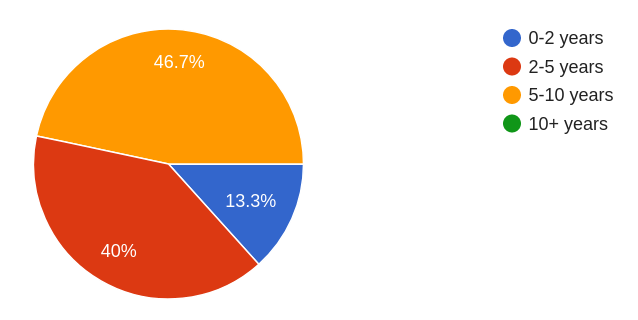
\includegraphics[width=10cm]{images/demographics-experience-cloud-native-crop1.png}
  \caption{Respondent experience in cloud-native architecture}
  \label{figure:experience-cna}
\end{figure}

\begin{figure}[h]\centering
  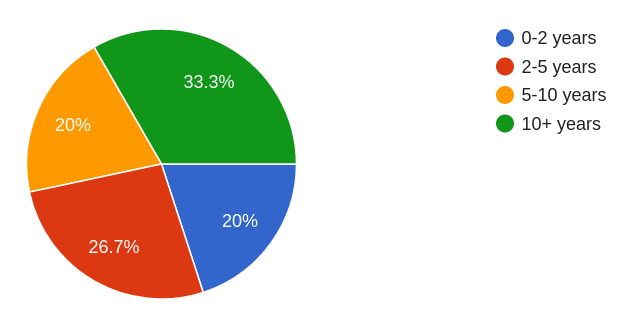
\includegraphics[width=10cm]{images/demographics-experience-software-architecture-crop1.png}
  \caption{Respondent experience in software architecture in general}
  \label{figure:experience-architecture}
\end{figure}

\begin{figure}[h]\centering
  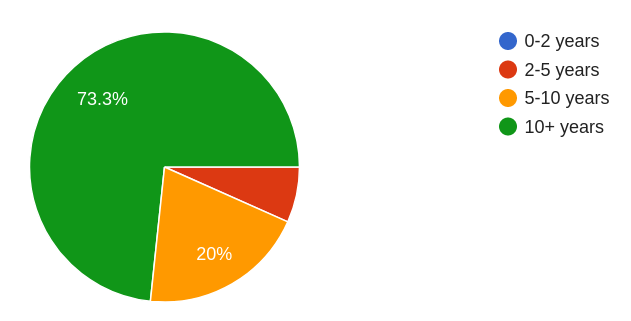
\includegraphics[width=10cm]{images/demographics-experience-information-technology-crop1.png}
  \caption{Respondent experience in information technology in general}
  \label{figure:experience-it}
\end{figure}

%%%%%%%%%%%%%%%%%%%%%%%%%%%%%%%%%%%%
\section{Prioritization of maintainability (Q4)}

To calculate a priority score for each quality attribute, I gave the options an
incremental integer value from 1 to 5. The value 1 corresponds to option
\textit{Least Important}, while value 5 corresponds to \textit{Most important}.
The absolute values chosen here are not of importance as long as the difference
between each consecutive option is equal, in order not to introduce additional
bias. This makes our scale analogous to the Likert scale \todo{ref?}, which is
often used for questionnaires in research.


\begin{table}[!h]
  \begin{center}
    \caption{Priority options and their numerical weights}
    \label{table:priorities1}
    \begin{tabular}{|c|c|}
      \hline
      \textbf{Priority} & \textbf{Weight} \\
      \hline
      Most important    & 5               \\
      More important    & 4               \\
      Important         & 3               \\
      Less important    & 2               \\
      Least important   & 1               \\
      \hline
    \end{tabular}
  \end{center}
\end{table}

Table \ref{table:priorities2} shows the average priorities and other relevant
metrics for the quality attributes.

\begin{table}[!h]
  \begin{center}
    \caption{Average priorities and other metrics for the quality attributes}
    \label{table:priorities2}
    \begin{tabular}{|c|c|c|c|c|}
      \hline
      \textbf{QA}     & \textbf{Average} & \textbf{Min} & \textbf{Mode} & \textbf{Max} \\
      \hline
      Security        & 4.07             & 1            & 5             & 5            \\
      Reliability     & 3.80             & 1            & 5             & 5            \\
      Maintainability & 2.67             & 1            & 2             & 4            \\
      Scalability     & 2.27             & 1            & 1             & 5            \\
      Performance     & 2.20             & 1            & 1             & 4            \\
      \hline
    \end{tabular}
  \end{center}
\end{table}


%%%%%%%%%%%%%%%%%%%%%%%%%%%%%%%%%%%%
\section{Ways to improve maintainability (Q5 \& Q6)}

\todo{%
  Extract suggestions, split to categories, present here, etc.
}

Some preliminary categorization of results:
\begin{itemize}
  \item Platform and technology choices
        \begin{itemize}
          \item Common technologies
          \item Managed services
          \item Infrastructure as Code (IaC)
          \item Configuration as Code (CaC)
          \item Continuous Integration and Continuous Deployment (CI/CD)
        \end{itemize}
  \item Application architecture
        \begin{itemize}
          \item Microservices Architecture (MSA)
          \item Statelessness
          \item Automatic scaling
          \item Modularity
          \item Loose coupling
          \item SOLID principles
        \end{itemize}
  \item Others (processes, philosophy, etc)
        \begin{itemize}
          \item DevOps
          \item Clear naming of resources
          \item Documentation
          \item Code reviews
          \item KISS principle
        \end{itemize}
\end{itemize}

%%%%%%%%%%%%%%%%%%%%%%%%%%%%%%%%%%%%
\section{Experience vs. prioritization of maintainability}

\todo{should be simple}

%%%%%%%%%%%%%%%%%%%%%%%%%%%%%%%%%%%%
\section{Experience vs. suggested ways to improve maintainability}

\todo{Slightly more involved. Which metrics to select?
  \begin{itemize}
    \item number of suggestions?
    \item popularity of suggestions in context of survey?
    \item popularity of suggestions in the wider context of existing research?
  \end{itemize}
}


%%%%%%%%%%%%%%%%%%%%%%%%%%%%%%%%%%%%%%%%%%%%%%%%%%%%%%%%%%%%%%%%%%%%%%%%%%%%%%
\chapter{Discussion}
\label{chapter:discussion}

In this section I further discuss the results presented in previous chapter.
\tmp{I also consider existing literature and contrast my results against
  findings of those who have researched the topic before me.}


In table \ref{table:priorities3} are listed the distances between the average
priorities. Distances are calculated from results shown in table
\ref{table:priorities2}. From these values we can draw multiple conclusions.
The top two quality attributes, Security and Reliability, are unequivocally the
most highly prioritized attributes in the minds of our cloud architects. The
distance between second and third most prioritized attributes is by far the
largest individual jump in values. Maintainability is sitting quite comfortable
in the middle of the range. This likely means it is considered important, but
not a priority if sacrifices need to be made to software quality. Performance
and scalability are considered least important items to an almost identical
degree.

\begin{table}[!h]
  \begin{center}
    \caption{Average priorities and delta to next highest item}
    \label{table:priorities3}
    \begin{tabular}{|c|c|c|}
      \hline
      \textbf{QA}     & \textbf{Average} & \textbf{$\Delta$} \\
      \hline
      Security        & 4.07             & -                 \\
      Reliability     & 3.80             & 0.27              \\
      Maintainability & 2.67             & 1.13              \\
      Scalability     & 2.27             & 0.40              \\
      Performance     & 2.20             & 0.07              \\
      \hline
    \end{tabular}
  \end{center}
\end{table}

%%%%%%%%%%%%%%%%%%%%%%%%%%%%%%%%%%%%%%%%%%%%%%%%%%%%%%%%%%%%%%%%%%%%%%%%%%%%%
\chapter{Conclusions}
\label{chapter:conclusions}


%%%%%%%%%%%%%%%%%%%%%%%%%%%%%%%%%%%%%%%%%%%%%%%%%%%%%%%%%%%%%%%%%%%%%%%%%%%%%%
\printbibliography

\nocite{*}
\todo{remove the nocite command from end of thesis.tex before submitting!}

%%%%%%%%%%%%%%%%%%%%%%%%%%%%%%%%%%%%%%%%%%%%%%%%%%%%%%%%%%%%%%%%%%%%%%%%%%%%%%
\appendix


\end{document}
